\chapter{EMMA} 
\label{chapter-5} 

Intro to goal of chapter. Make sure they understand it is my contribution. Use active voice.

%----------------------------------------------------------------------------------------
%	SECTION 
%----------------------------------------------------------------------------------------

\section{Problem Statement}

Hypothesis. What and why.
\begin{itemize}
\item no sequence
\item no image
\item MLP dimension $D_i$ 
\item ...\\
\end{itemize}

Explain notation. $\{\mathbf{x}_1, \ldots, \mathbf{x}_M\}$ $M$ modes and $N \times D_i$ matrices, $\mathbf{y}$, $\hat{\mathbf{y}}$ loss ... Only makes sense if MI lower or equal MI. Explain with diagram.
\begin{figure}[!h]
\centering
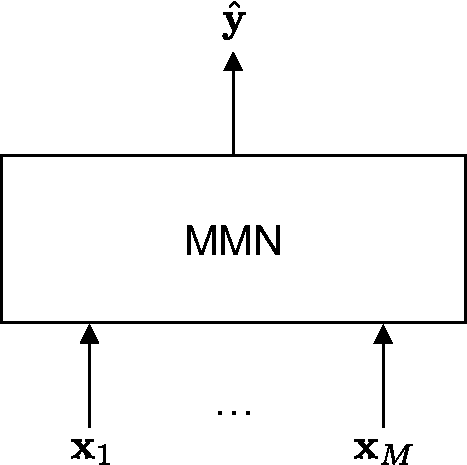
\includegraphics[scale=0.5]{figures/mlp-without-emma}
\caption{blabl}	
\label{fig:summary}
\end{figure}

If outlying data (often the case in real world to a certain degree) then MI drops, we cannot do anything to that however in DL it is worse the accuracy drops even more than it loses information (high activations if noise or unknown). Another problem is the fact that DL makes prediction even when big loss of information and does not indicate it is less certain. We can solve this with EMMA it basically determines a $\beta_i$ for each mode between zero and one. The problem about uncertainty will be explained later. explain with diagram.
\begin{figure}[!h]
\centering
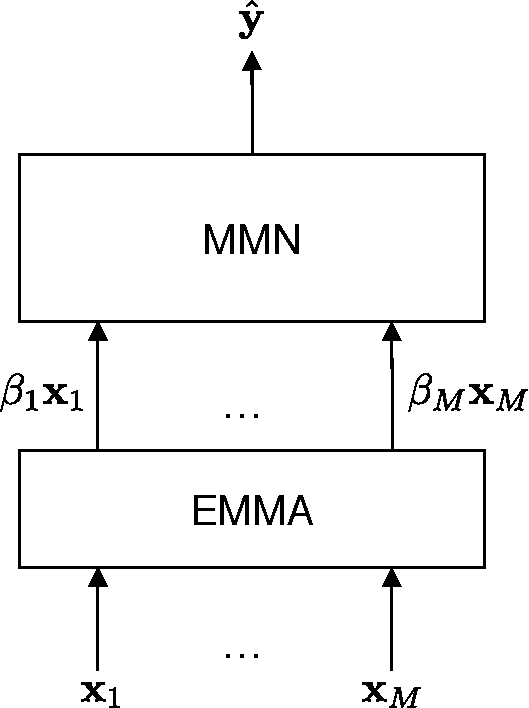
\includegraphics[scale=0.5]{figures/mlp-with-emma}
\caption{Summary}	
\label{fig:summary}
\end{figure}

How compute/determine $\beta$, see next section

%----------------------------------------------------------------------------------------
%	SECTION 
%----------------------------------------------------------------------------------------

\section{General Framework}

What is importance, what do we mean by this. Motivate why determine importance. Three things influence importance:
\begin{itemize}
\item Out-of-distribution: the more unknown, the less accuracy, the less important
\item Relevance: at the same, some carry more information for prediction or less
\item Independence: how independ with others, are two modes very coupled and carrying the same information and thus redundant (one noisy, other takes over) or completely independent (not easy to completely dismiss info of a noisy mode in that case)
\end{itemize}
Start with potential satisfies first one (out of distrib). Imagine if we create a new energy taking potential but also relevance and independence. We call this modal energies. And has the following form. Loosely inspired from Boltzmann machines. Explain f is relevance (influence by optim algorithm, minimize loss) and g (how to explain???)
$$f(\Psi) + \sum g(\Psi)$$
\indent Link $E_i$ to importance scores via gibbs distribution. Interpretability $\alpha_i$. (How to explain??)\\
Idea of attention is selection but at the same time capactiy. Model learns an optimal capactiy for the task. How much information it needs to led pass by. (How to explain?) \\

In summary, quick review from start to end. Details explain in each section.
\begin{figure}[!ht]
\centering
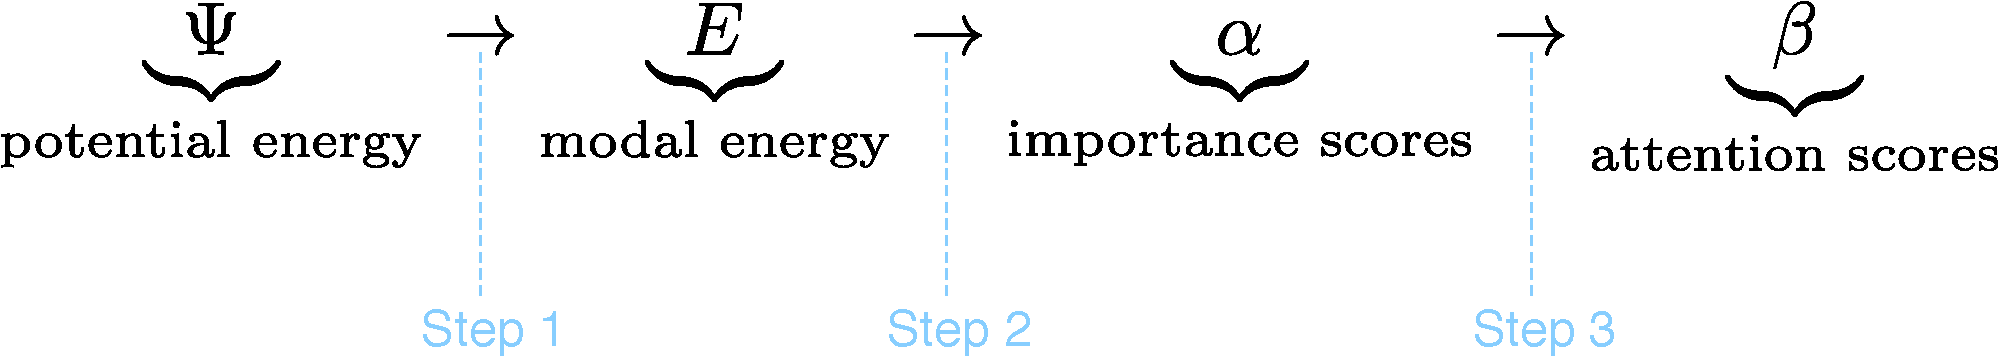
\includegraphics[scale=0.4]{figures/framework}
\end{figure}

%----------------------------------------------------------------------------------------
%	SECTION 
%----------------------------------------------------------------------------------------

\section{Step 1}
One paragraph per item.
\begin{itemize}
\item Mention room from improvement, multiple other ways
\item Correction. Minimum potential. Max because log gradient. $\Psi'$.
\item Self-energy $e_i$. Shape.
\item Shared energy $e_{ij} = e_i^{\gamma_{ij}}e_j^{1-\gamma_{ij}}$. Symmetry, coupling.
\item Modal energy (Boltzmann) self + shared.
\item Notice system energy. Interpretation.
\end{itemize}

%----------------------------------------------------------------------------------------
%	SECTION 
%----------------------------------------------------------------------------------------

\section{Step 2}

\begin{itemize}
\item Gibbs distribution short with $\mathcal{C} = \frac{1}{T}$, high temperature (low coldness) then ... and low temperature (high coldness) ... (explain intuitive influence with diagrams.  
\item Hyperparameter tuned because can have influence on accuracy. Explain what temperature really is (a way of tuning the strictness, better explain??)
\item Mention annealing
\end{itemize}

\begin{figure}[!h]
\centering
\begin{subfigure}{.5\textwidth}
  \centering
  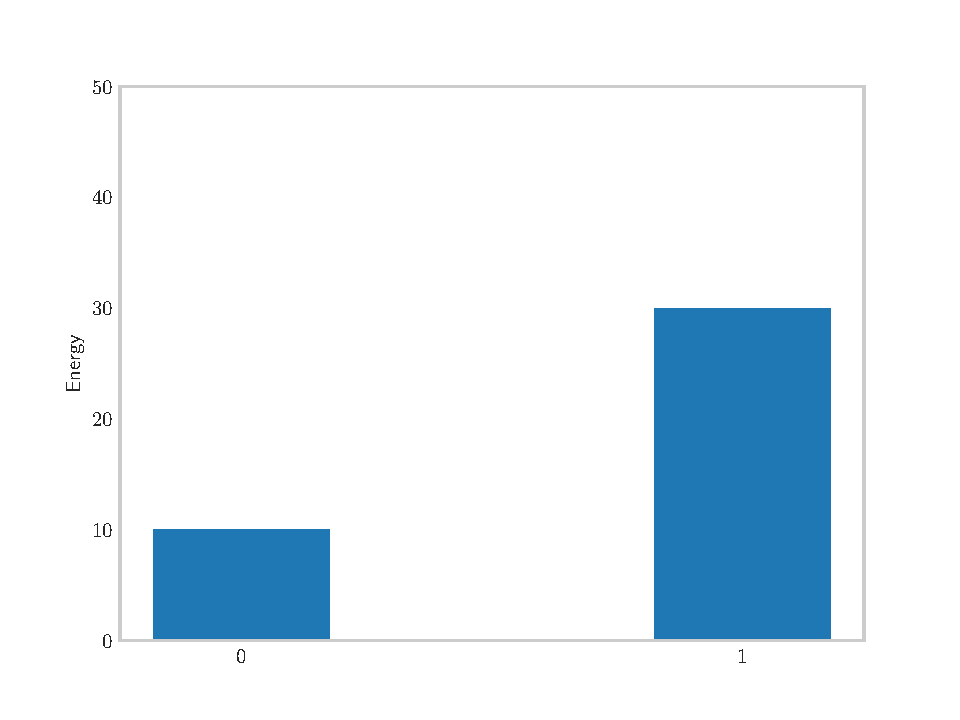
\includegraphics[width=.75\linewidth]{figures/input-gibbs}
  \caption{Autoencoder}
  \label{fig:ae}
\end{subfigure}%
\begin{subfigure}{.5\textwidth}
  \centering
  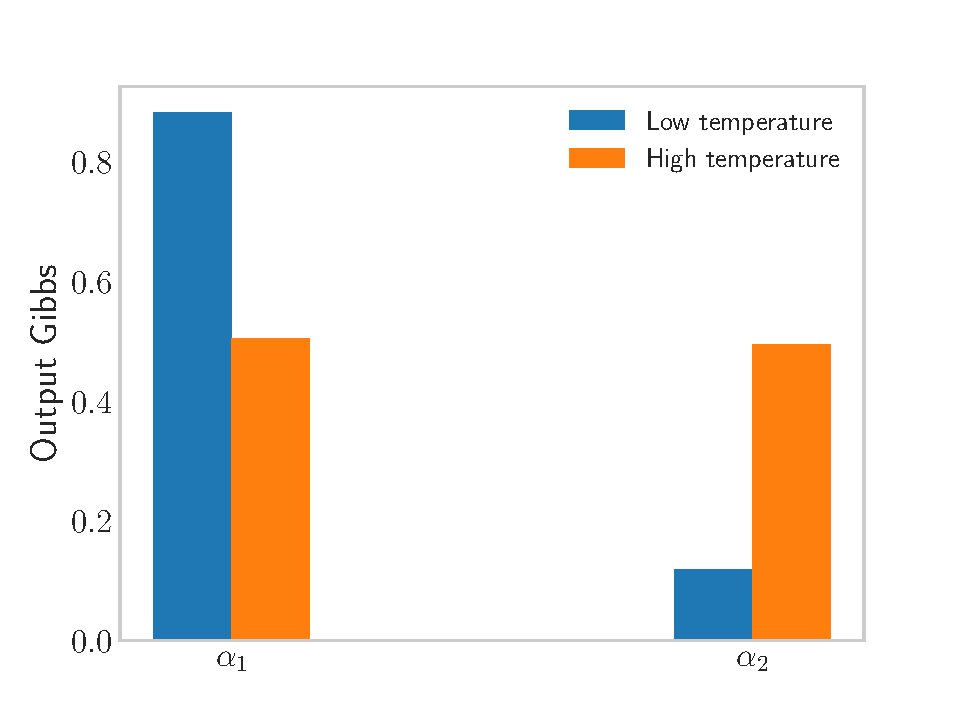
\includegraphics[width=.75\linewidth]{figures/result-gibbs}
  \caption{Data space}
  \label{fig:ae-process}
\end{subfigure}
\caption{Reconstruction}
\label{fig:test}
\end{figure}


%----------------------------------------------------------------------------------------
%	SECTION 
%----------------------------------------------------------------------------------------

\section{Step 3}
Every item is one subsection. First one without header title.
\begin{itemize}
\item Show formula + explain main points design
	\begin{itemize}
	\item tanh
	\item relu
	\item $g_a > 0$ and $b_a \in [0,1]$
	\item common (explain later in subsection)
	\end{itemize}
\item Energy threshold
\item Capacity. What is it intuitively. Math derivation (uninteresting part in appendix, complete version). Small paragraph on intuitive difference with temperature with analogy (fun), notice one is tuned and other is learned, trade-off between the two (crossing).
\item Asymmetric effect. most of time attention is $\tanh(\mathbf{Wx} + \mathbf{b})$, in this case gain and bias are not common. We have a problem if this is not common -- assymetry.
\end{itemize}

\begin{figure}[!h]
\centering
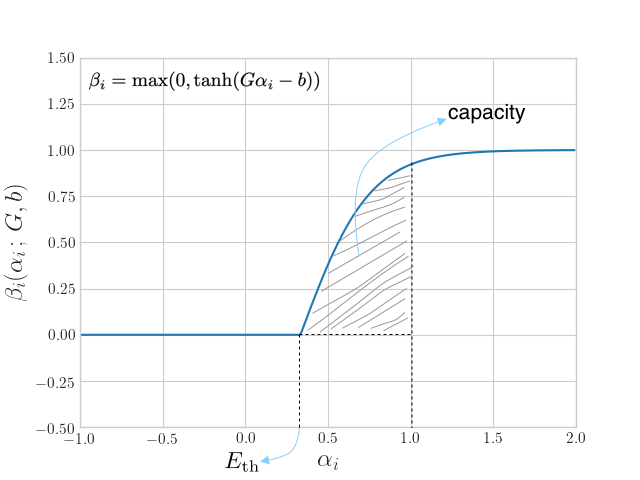
\includegraphics[scale=0.36]{figures/tanh-annotated}
\caption{Summary}	
\label{fig:summary}
\end{figure}

%----------------------------------------------------------------------------------------
%	SECTION 
%----------------------------------------------------------------------------------------

\section{Training \& Regularization}

\begin{itemize}
\item Explain training, 2 phases, train with corrupted/unsee data let us say 50/50 but depend on application.
\item The problem is - loose of interpretation because (how to explain??). This is why we add a regularizer. Explain $\xi_i$ (replace $\eta(m_k)$ by $\xi_k$). Math expression. Explain intuitively and lambda. Quite intuitive, however as we will see some care needs to be taken. Phenomenon in particular case.
\end{itemize}
\subsection*{Backpropagation of regularizer}
\begin{itemize}
\item param step update $\theta - \epsilon\lambda\nabla_\theta\Omega$
\item develop $\nabla\Omega$, stop before $M'$ introduction
\item explain what happens for bad choice of $M'$ and for good choice $M'$
\end{itemize}
\subsection*{Contrastive divergence}
Explain two cases. No itemize. Illustrations.


%----------------------------------------------------------------------------------------
%	SECTION 
%----------------------------------------------------------------------------------------

\section{Summary}

Describe diagram summarizing end-to-end in two phases with gradients. 
\begin{figure}[!h]
\centering
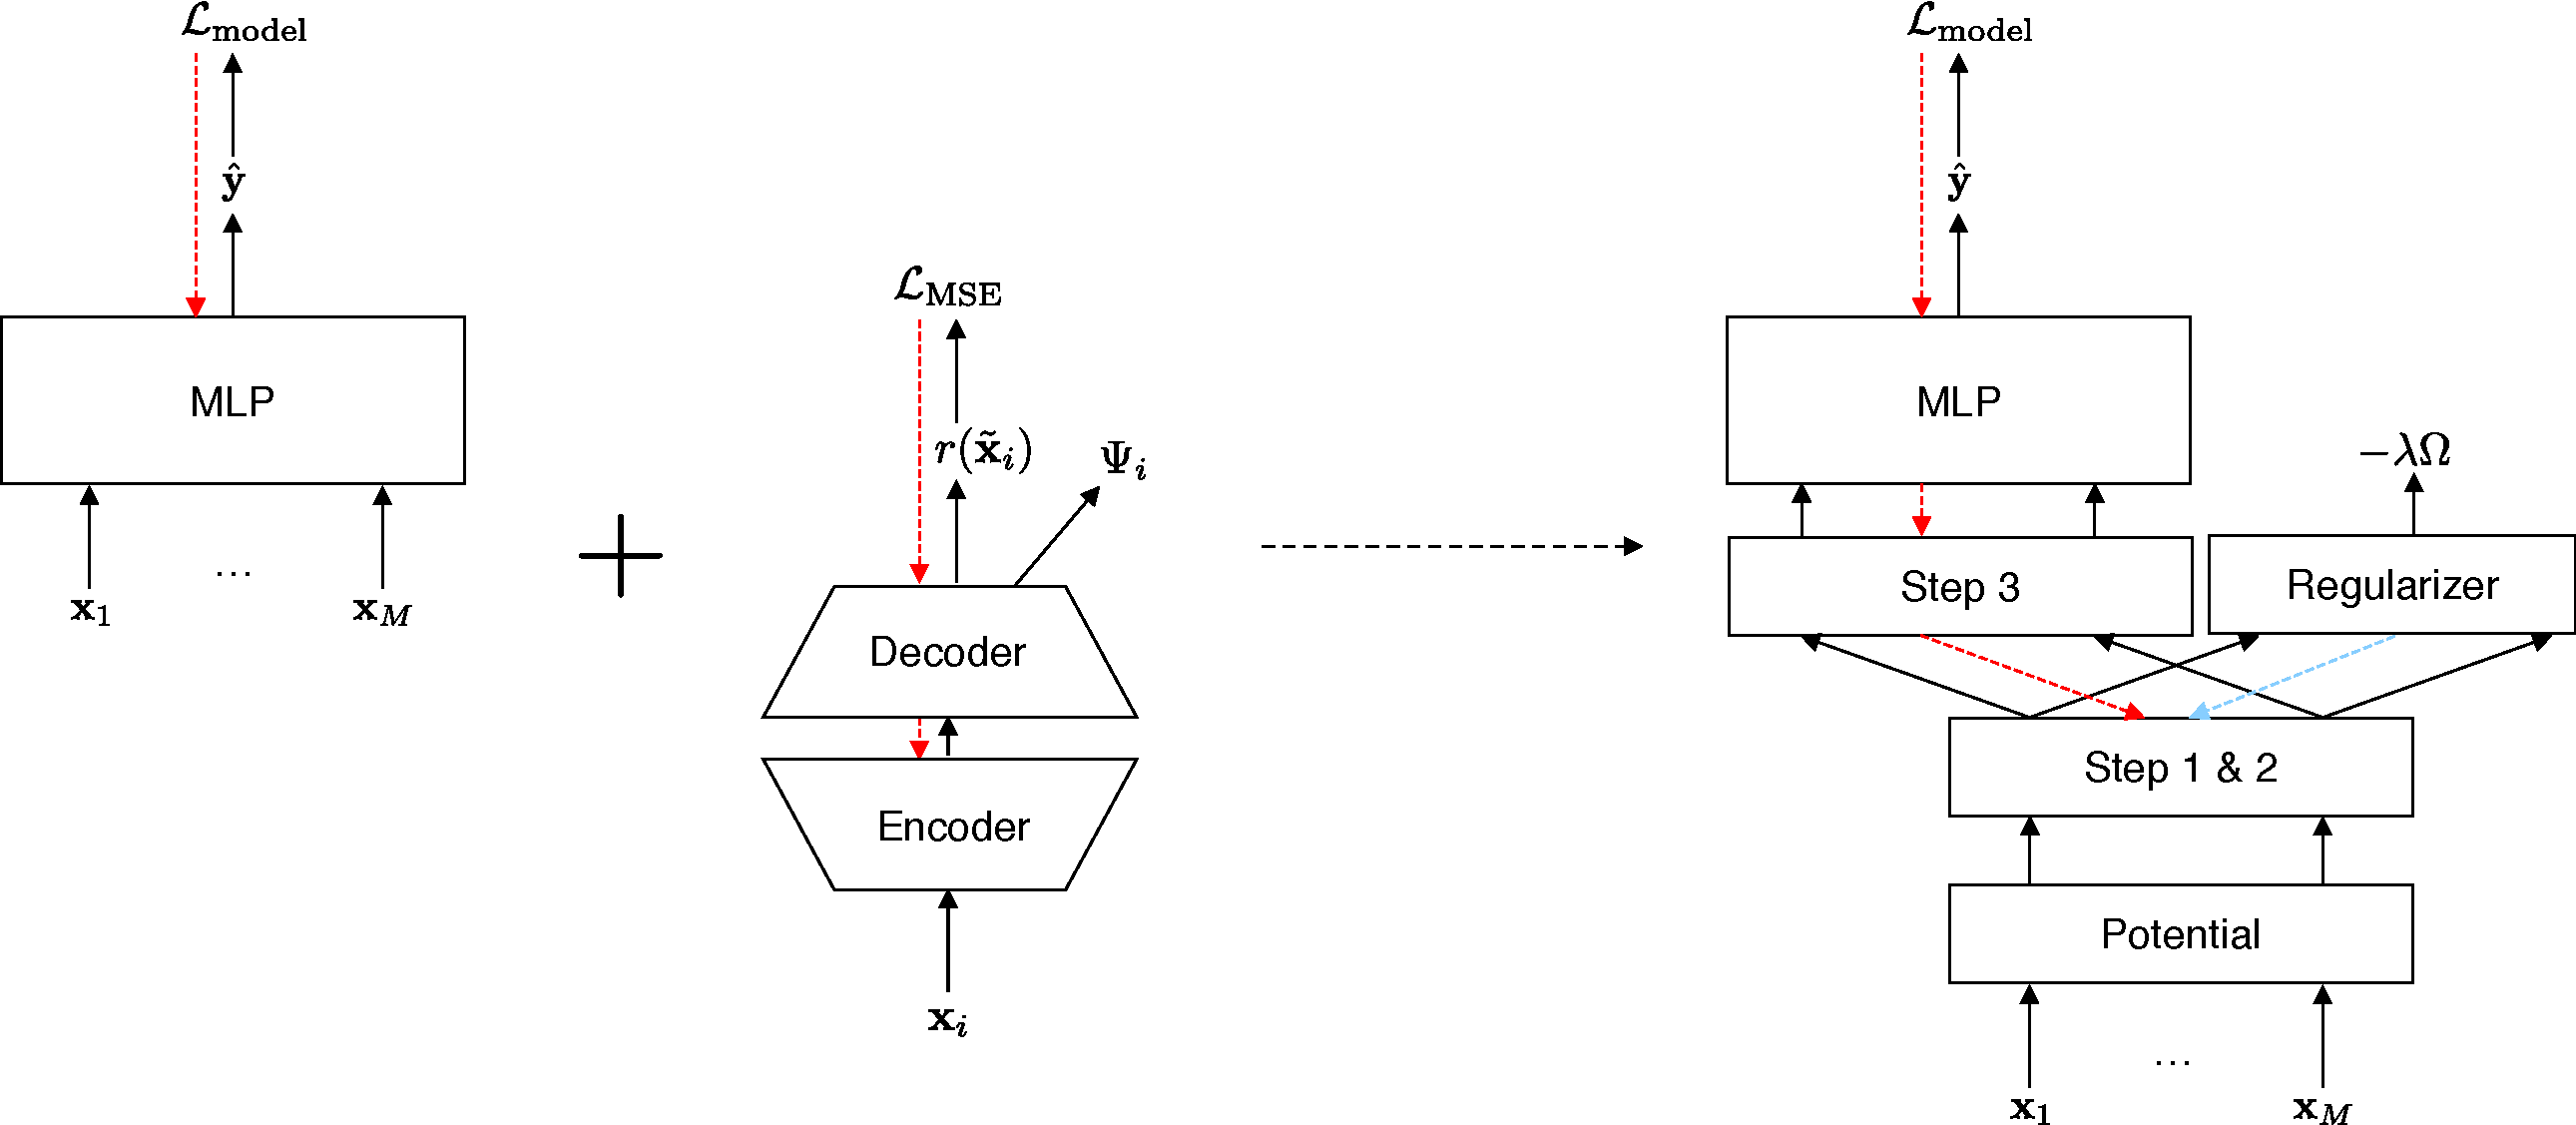
\includegraphics[scale=0.36]{figures/summary-training}
\caption{Summary}	
\label{fig:summary}
\end{figure}

%----------------------------------------------------------------------------------------
%	SECTION 
%----------------------------------------------------------------------------------------

\section{Research questions}
\begin{itemize}
\item does EMMA improve robustness of model, not only on corrupted data. But on more corrupted data, and unseen data. In other words does it robustness generalize.
\item does EMMA help with interpretability (E, alpha, gamma)
\item what is the tradeoff between interpretability (lambda) and accuracy
\item what is the tradeoff between temperature and capacity? Do we need to minimize capacity to generalize robustness?
\end{itemize}